%%%%%%%%%%%%%%%%%%%%%%%%%%%%%%%%%%%%%%%%%
% Predicting the outcome of online multiplayer  Heroes of the Storm Matches
% Author: Jesse Swidler
% Date: October 2017
% For Udacity Machine Learning Nanodegree
%
%
% The original template for the paper was acquired from http://www.LaTeXTemplates.com and the original
% license from the template is below:
% Journal Article
% LaTeX Template
% Version 1.4 (15/5/16)
%
% This template has been downloaded from:
% http://www.LaTeXTemplates.com
%
% Original author:
% Frits Wenneker (http://www.howtotex.com) with extensive modifications by
% Vel (vel@LaTeXTemplates.com)
%
% License:
% CC BY-NC-SA 3.0 (http://creativecommons.org/licenses/by-nc-sa/3.0/)
%
%%%%%%%%%%%%%%%%%%%%%%%%%%%%%%%%%%%%%%%%%

%----------------------------------------------------------------------------------------
%	PACKAGES AND OTHER DOCUMENT CONFIGURATIONS
%----------------------------------------------------------------------------------------

\documentclass[twoside,twocolumn]{article}

\usepackage{blindtext} % Package to generate dummy text throughout this template 

\usepackage[sc]{mathpazo} % Use the Palatino font
\usepackage[T1]{fontenc} % Use 8-bit encoding that has 256 glyphs
\linespread{1.05} % Line spacing - Palatino needs more space between lines
\usepackage{microtype} % Slightly tweak font spacing for aesthetics



\usepackage[english]{babel} % Language hyphenation and typographical rules

\usepackage[hmarginratio=1:1,top=32mm,columnsep=20pt]{geometry} % Document margins
\usepackage[hang, small,labelfont=bf,up,textfont=it,up]{caption} % Custom captions under/above floats in tables or figures
\usepackage{booktabs} % Horizontal rules in tables

\usepackage{lettrine} % The lettrine is the first enlarged letter at the beginning of the text

\usepackage{enumitem} % Customized lists
\setlist[itemize]{noitemsep} % Make itemize lists more compact

\usepackage{abstract} % Allows abstract customization
\renewcommand{\abstractnamefont}{\normalfont\bfseries} % Set the "Abstract" text to bold
\renewcommand{\abstracttextfont}{\normalfont\small\itshape} % Set the abstract itself to small italic text

\usepackage{titlesec} % Allows customization of titles
\renewcommand\thesection{\Roman{section}} % Roman numerals for the sections
\renewcommand\thesubsection{\roman{subsection}} % roman numerals for subsections
\titleformat{\section}[block]{\large\scshape\centering}{\thesection.}{1em}{} % Change the look of the section titles
\titleformat{\subsection}[block]{\large}{\thesubsection.}{1em}{} % Change the look of the section titles

\usepackage{fancyhdr} % Headers and footers
\pagestyle{fancy} % All pages have headers and footers
\fancyhead{} % Blank out the default header
\fancyfoot{} % Blank out the default footer
\fancyhead[C]{Predicting HotS Matches $\bullet$ October 2017 $\bullet$ Udacity MLND} % Custom header text
\fancyfoot[RO,LE]{\thepage} % Custom footer text

\usepackage{titling} % Customizing the title section

\usepackage{hyperref} % For hyperlinks in the PDF

\usepackage[capposition=top]{floatrow}
\usepackage{mathtools}
\usepackage{graphicx}
\graphicspath{ {images/} }

\usepackage{adjustbox}
%----------------------------------------------------------------------------------------
%	TITLE SECTION
%----------------------------------------------------------------------------------------

\setlength{\droptitle}{-4\baselineskip} % Move the title up

\pretitle{\begin{center}\Huge\bfseries} % Article title formatting
\posttitle{\end{center}} % Article title closing formatting
\title{Predicting the outcome of online \textit{Heroes of the Storm} Matches} % Article title
\author{%
\textsc{Jesse Swidler} % Your name
\normalsize \href{mailto:jswidler@gmail.com}{jswidler@gmail.com} \\ % Your email address
\normalsize Udacity MLND Capstone Project % Your institution
%\and % Uncomment if 2 authors are required, duplicate these 4 lines if more
%\textsc{Jane Smith}\thanks{Corresponding author} \\[1ex] % Second author's name
%\normalsize University of Utah \\ % Second author's institution
%\normalsize \href{mailto:jane@smith.com}{jane@smith.com} % Second author's email address
}
\date{October 2017} % Leave empty to omit a date
\renewcommand{\maketitlehookd}{%
\begin{abstract}
\noindent
Heroes of the Storm is an online multiplayer game where teams of five players choose heroes with different abilities and play against each other.  Machine learning techniques were used in an attempt to predict the outcome of a match by using known data about the players and the heroes they choose.  Various neural network architectures and methods of serializing each game into features were tested to maximize the ability to predict game outcomes.  An overall accuracy of 62.1\% is achieved.  Some games are found to be easier to predict than other games, such that 18.8\% of games can be predicted with 70\% confidence or above, and 51.8\% of games can be predicted with greater than 60\% confidence.
\end{abstract}
}

%----------------------------------------------------------------------------------------

\begin{document}

% Print the title
\maketitle

%----------------------------------------------------------------------------------------
%	ARTICLE CONTENTS
%----------------------------------------------------------------------------------------

\section{Introduction}

\lettrine[nindent=0em,lines=2]{H}{eroes of the Storm}\normalfont\ is an online video game made by \textbf{Blizzard Entertainment}.  In the game, two teams of five human players choose heroes with unique abilities and battle against each other in a battle arena, giving rise to the acronym for the genre - \textbf{MOBA}, or \textbf{M}ultiplayer \textbf{O}nline \textbf{B}attle \textbf{A}rena.  In the most popular mode, each team has a number of structures, of which the most important is the keep.  Players work together with each other and waves of non-player characters to advance on the map and ultimately destroy the opposing team's keep.

In this game mode, players can play against each other in ranked and unranked play.  \textbf{Blizzard} keeps track of how a player performs and calculates a skill rating for the each player which is used to match up players of equal skill.  In my experience, the matchmaking is fair as I have won very close to half of the games that I play.

\textbf{Blizzard Entertainment} does not yet provide an easy way to download a history of games played.  However, \textbf{HOTSLogs} is a website devoted to keeping stats on \textit{Heroes of the Storm} players (https://www.hotslogs.com/).  Many players choose to upload replay files to this website, which then analyzes the games and provides statistics, such as which heroes are most likely to win, which players are the best, or which talents (unlocked by leveling up in each game) perform best.  \textbf{HOTSLogs} provides a simple way to download a summary of the last 30 days of games, which will provide the data for this project.

\section{Goals}

The goal of the project is to develop a classifier capable of predicting the odds of a team winning a \textit{Heroes of the Storm} match.

Using \textbf{Keras}, we will build a network to complete this task.  The problem is one of binary classification - given \textbf{Team A} and \textbf{Team B}, will \textbf{Team A} win?  We will use log loss to measure the performance of the model during training.  This make sense because the problem is one of binary classification, and it will help make sure the model developed is well calibrated - it must not only say which team is most likely to win, but also how likely that team is to win.

After training, we will measure the accuracy and calibration of the model.  The best model should have the highest accuracy.

For comparison, we will also feed the data into a naive bayesian classifier. This was decided after noticing patterns in the dataset which would make bayesian learning applicable.  We use \textbf{GaussianNB} from \textbf{sklearn} to perform this task.

%------------------------------------------------

\section{Dataset}

The dataset from \textbf{HOTSLogs} can be obtained at https://www.hotslogs.com/Info/API.  The dataset will contain the last 30 days of games, which is a good starting point for a project like this.  

We would like to use as much data as possible, as we expect more examples will improve our ability to predict the game outcomes.  For the most data, we should set the window as far back as possible.  But the game also receives regular updates which adds new heroes, new maps, and changes the relative strength of heroes.  This means we would need to recognize the temporal nature of old results if we used data from old game patches.  By using recent data, we can simplify our model to only predict the outcome of games for the current patch.  The ease of obtaining recent 30 day exports from \textbf{HOTSLogs} will therefore help to solidify our choice of using a 30 day window of game data for training the model.

The dataset used in the analysis done by this paper was dated October 19, 2017.  It contained 1,954,853 games.

The dataset contains three \textit{csv} files.  Games are described by 10 rows in one \textit{csv} and 1 row in another.  The dataset will be rewritten before processing so each game is represented by a single row in a different \textit{csv}.

\subsection{Game Modes}

\begin{table}[h]
\caption{Game Modes}
\label{table:modes}
\centering
\begin{tabular}{lr}
\toprule
Game Mode & Number of Games \\
\midrule
Quick Match & 1,340,645  (68.58\%) \\
Hero League  & 333,147  (17.04\%) \\
Team League & 139,252  (7.12\%) \\
Unranked Draft & 141,809  (7.25\%) \\
\midrule
Total & 1,954,853 \\
\bottomrule
\end{tabular}
\end{table}

There are four different game modes in the dataset. See Table \ref{table:modes}.  All of these game modes are actually the same game played with the same rules following hero selection.  In \textit{quick match}, players pick a hero to play, and the matchmaker forms supposedly balanced teams.  In the other three modes, there is a hero draft which occurs after players have been put onto teams.  During the draft, players take turns choosing their hero.  The difference in these three modes is that there is public ranking for \textit{hero league}, which is played alone, and \textit{team league}, which is played with groups of 2, 3, or 5; while \textit{unranked draft} has no public leader board.

Players have an independent \textbf{Match Making Ranking (MMR)} for each mode which is used by the matchmaker regardless of whether or not the leaderboard is public.  This hidden MMR is used so that both teams in a game should be evenly matched.

\subsection{Maps}

\begin{table}[h]
\caption{Maps}
\label{table:maps}
\centering
\begin{tabular}{lr}
\toprule
Map & Number of Games \\
\midrule
Battlefield of Eternity & 177,817  (9.10\%) \\
Blackheart's Bay & 178,621  (9.14\%) \\
Cursed Hollow & 186,238  (9.53\%) \\
Dragon Shire & 179,348  (9.17\%) \\
Garden of Terror & 151,163  (7.73\%) \\
Haunted Mines & 122,055  (6.24\%) \\
Infernal Shrines & 149,708  (7.66\%) \\
Sky Temple & 176,877  (9.05\%) \\
Tomb of the Spider Queen & 152,249  (7.79\%) \\
Towers of Doom & 153,367  (7.85\%) \\
Braxis Holdout & 177,095  (9.06\%) \\
Warhead Junction & 150,315  (7.69\%) \\
\midrule
Total & 1,954,853 \\
\bottomrule
\end{tabular}
\end{table}

The dataset has 20 maps listed in it.  I do not think that all the maps which have names and map ids assigned are actually playable in the game.  In addition, all of the matchmaking modes use the same limited pool of maps, called the \textbf{map rotation}, which changes every few weeks.  So during a 30 day period, some maps are never played in the dataset.  In this set, there are 12 maps with games played on them. See Table \ref{table:maps}.  Only these 12 maps will be considered while training the model.

\subsection{Heroes}

The dataset has 73 heroes listed in it - but there is only 1 game recorded with Ana and no games with Junkrat.  These are the two most recently released heroes at the time of writing.  Because there is virtually no data for either of them in the dataset, they will not be considered, and we will train the model as if there are 71 heroes to choose from.

71 heroes provides many many different match up possibilities.  We can calculate how many unique matchups there are in \textit{quick match} using equation \ref{equation:qmmatchups} and the three draft modes using equation \ref{equation:draftmatchups}.  There are more possible combinations in \textit{quick match} because the same hero can be on both teams, which cannot happen when there is a draft. 

\begin{equation}
\label{equation:qmmatchups}
\begin{aligned}
matchups_{qm} &= \frac{{71 \choose 5}\times({71 \choose 5}-1)}{2} + {71 \choose 5} \\
&= 84,759,021,694,095 \\
&\approx{8.48e13}
\end{aligned}
\end{equation}

\begin{equation}
\label{equation:draftmatchups}
\begin{aligned}
matchups_{draft} &= \frac{{71 \choose 5}\times{71-5 \choose 5}}{2} \\
&= 58,178,994,649,776 \\
&\approx{5.82e13}
\end{aligned}
\end{equation}

We find there are more than 84 trillion possible matchups for \textit{quick match} and over 58 trillion for the other modes when only hero selection is considered.

Some heroes are more likely to win than others.  The top and bottom five heroes, sorted by win, are listed in Table \ref{table:winpercent}.

\begin{table}[h]
\caption{Top and Bottom Five Heroes by Win Percent}
\label{table:winpercent}
\centering
\begin{tabular}{lr}
\toprule
Hero & Win Percent \\
\midrule
Murky & 55.6\% \\
Azmodam & 55.4\% \\
Samuro & 55.3\% \\
Nazeebo & 54.8\% \\
Zagara & 53.6\% \\
\dots \\
Alarak & 45.2\% \\
Tychus & 45.0\% \\
Garrosh & 44.7\% \\
Chromie & 43.8\% \\
Medivh & 37.9\% \\
\bottomrule
\end{tabular}
\end{table}


The game breaks heroes down into four classifications: \textbf{Warrior}, \textbf{Specialist}, \textbf{Support}, and \textbf{Assassin}.  \textbf{HOTSLogs} breaks down heroes further into 9 subgroups:  \textbf{Ambusher},  \textbf{Bruiser},  \textbf{Burst Damage},  \textbf{Healer},  \textbf{Siege},  \textbf{Support},  \textbf{Sustained Damage},  \textbf{Tank}, and  \textbf{Utility}.  These labels are useful for describing how a hero is expected to be played.  

\begin{table*}
\caption{Composition Matchups}
\label{table:compmatchup}
\centering
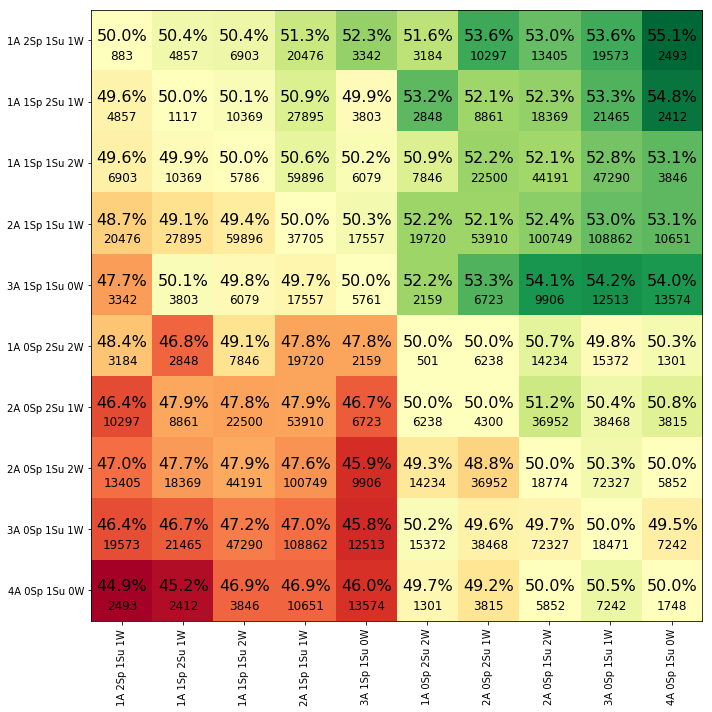
\includegraphics[width=\textwidth]{compmatchup}
\floatfoot{\textit{Analysis of all the games in the dataset set shows that some team compositions are stronger than others.}  Top percentage shows probability the composition on the left will beat the composition on the bottom.  Bottom number is the total number of games which were played with this matchup.  \textbf{A=Assassin, Sp=Specialist, Su=Support, W=Warrior}, for instance \mbox{\textbf{1A 2Sp 1Su 1W}} means the team had one assassin, two specialists, one support, and one warrior.}
\end{table*}

The most competitive teams will use a variety of heroes.  This is illustrated in an interesting way in Table \ref{table:compmatchup}.  The team compositions are grouped by the number of heroes in each of the four hero groups on the team, and compared against each other.  As expected, hero choice matters in determining who will win.  For instance, a team without any support heroes does much worse than teams with all four groups.  However, even in unbalanced matchups, there is still a reasonable chance for the "weaker" group composition to have won.

\subsection {Players}
\label{players}

The dataset contains information on how each player performed in each game.  Most of that data is ignored by our model, as it describes what happened during the game, such as how much damage or how much healing a player caused.  There are three attributes from each player which are known before the game which is potentially available to the matchmaker or though the \textbf{HOTSLogs} API.

\begin{itemize}
\item the hero the player choose
\item the player's level with that hero
\item the player's MMR when the game begins
\end{itemize}

The hero is identified by the hero id; 1-71.  The player's level with a hero is roughly approximate to how many games the player has played the specific hero in the past.  The player's MMR is not the same MMR used by \textbf{Blizzard}'s matchmaker, but is instead a \textbf{HOTSLogs} derived number, which should still measure the player's overall skill, although some game data might be missing.

Some outliers in this data was found.  The most obvious one is that some games had players who did not have a known MMR or hero level.  Another case was players with very low or very high MMRs.  Rather than deal with the added complexity of dealing with these edge cases with different properties from the games that most people play, they were filtered from the dataset.  This resulted in 203,002 games being filtered, reducing the overall size of the dataset by 10.4\% and leaving 1,751,851 games to train with.


%------------------------------------------------

\section{Methods}

In order to find the best classifier, a number of different approaches were used.  One problem was to figure out how to encode the initial dataset into a vector that can be interpreted by different machine learning algorithms.  Another problem was to discover what the best  architecture for interpreting that data would be.

\subsection{Initial Modeling}

Two models were created to experiment with the data.  A naive bayesian classifier was used as a benchmark model and provided a quick way of determining if a particular feature encoding contained information that could be used to predict game outcomes.  A neural net was found to consistently outperform the naive bayesian classifier, and was also used to test different feature encodings.

I choose to use a naive bayes classifier after noticing patterns such as certain heroes being more likely to win, and certain team compositions being more likely to win.  Both of these attributes suggest a bayesian classifier will perform with better than 50\%.

I played with neural network architectures just a small amount before attempting to optimized the feature encoding.  I found a two layer network with two hidden layers  with 500 perceptrons each performed favorably to the bayes classifier, and proceeded to test with it.  I also added dropout layers to prevent overfitting.

\subsection{Initial Feature Selection}

Ideally there would be 32 known features per game.  There are three known features per player, as previously discussed, as well as the game mode and map.  The problem with this is that the hero IDs, game mode, and map are all categorical labels, which will not work well with many machine learning techniques.

One possible solution to this issue is to use one hot encoding on all the categorical features.  If we were to do this, the ten hero selections would change into 710 separate features.  If we do not care which player picked which hero, we can instead encode each team in a separate 71 feature vector, as each hero can only appear once per team. 

I did not want to lose information about how good and experienced the player was with their hero, as some heroes are much harder to play than others.  I decided to add this information directly into the hero selection feature.  Because we have two pieces of information about each player, their MMR and their hero level, I split each possible hero choice into two features per team.  The labels for these features are things like \textit{a\_herommr\_Rexxar} and \textit{a\_herolevel\_Rexxar}.  The first character of the labels is either \textit{a} or \textit{b} depending on which team the player on.  If a hero is present on a team, the player's MMR and hero level is filled into the column.  For heroes which are not on the team, the values are set to zero.  With 71 heroes, this is 142 features per team and 284 features per game.

The maps and game modes are one hot encoded, which adds 12 and 4 additional features respectively, bringing the total to 300 features.  With these 300 features, everything about the game we know is included.

\subsection {Feature Experiments}

Other ways of creating features were tried in an attempt to increase the signal form the dataset.  The previous 300 features are sparse, and I expected there would be better ways to describe the game.

One successful improvement was to add features which contained the number of each type of hero on each team.  This was tried with group labels, subgroup labels, and artificially created labels that were generated through PCA (principal component analysis) of hero stats and a clustering algorithm.  The automatically generated labels also helped improve the prediction rates, however for the most part, no labels out performed subgroups, and there was little to no improvement when multiple typings were used in my experiments.  In the final model, we retain the subgroup counts.  There are 9 subgroups, so a total of 18 features are added to the inputs.

Another set of features which was tried and retained is a separate set of columns where player mmrs and levels are listed.  These features were given column names like \textit{a\_playerlevel\_1} and \textit{a\_playermmr\_1}.  The features have the exact same values as their respective herolevel and herommr columns. I suspect a direct comparison of how skilled the players are is useful in making predictions, but the information is generally too spread out in the sparse team vector for the information to be interpreted that way.  Adding 10 extra features per team to hold this information helped the classifiers find the information.

All together, there are 338 features which were fed into the final model.

One experiment which did help the benchmark model, but did not help the neural network, was to use PCA to change each hero into a number of dimensions.  By doing this, we can reduce the number of inputs needed to describe the team.  If we use five dimensions per hero, we can describe a team using 35 features (25 for the team, 5 for mmrs, and 5 for levels), instead of 142.  This encoding allowed the benchmark to exceed 57\% accuracy, an improvement of 0.5\%, and may have helped the neural network when only a subset of the dataset was being used for training.  Once enough data was being used for training purposes, any improvement from PCA features disappeared, I so I ultimately decided not to include them in the final model.

\begin{figure}
\caption{Heroes plotted against the first three principal components and colored by their \textbf{HOTSLogs} subgroup label}
\label{figure:heropca}
\centering
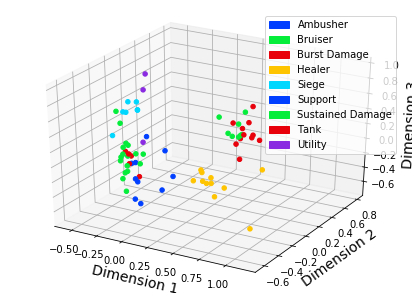
\includegraphics[width=\linewidth]{heropca}
\end{figure}

\subsection{Feature Normalization}

As the weights of each of the features vary quite a bit, they must be normalized.  Initially I used algorithms to automatically scale all the values to between 0 and 1.  However this required taking more than one pass over the data, and the process of converting the initial dataset into something that could be used by machine learning was slow.  It also meant it was difficult to batch things, as the normalized values would be scaled differently depending on what the min and max values were for that batch.  I eventually decided to set a custom scale for all the features.  This scaling happens during the first pass over the HOTSLog data when converting each game to a one dimensional array.

This is also nice because an application which uses the final model will have known formulas to apply to convert live inputs into the proper scale.

\subsection{Dataset Size}

Due in large part to the way the code is written, it takes a long time to export all 1.9 million games.  I have optimized it a bit since testing began, but it still takes over 2 hours to preprocess the entire dataset.  In order to test different ways of encoding the data, I would only preprocess some of the data and train on that.  This led to an early observation that more training data led to better results.

This showed up in different ways throughout my testing.  A good illustration of this occurs when doing K-fold validation on different models.  Using more folds meant more data would be used to train and less to validate, and accuracy would go up.  I initially was using far less of the dataset, but it became clear it would be a good idea to use as much of the dataset as possible.

\subsection{Model Hyperparameters}

Once I was satisfied with the data preprocessing step, I turned my attention to optimizing the model more.  The features considered for optimization were:

\begin{itemize}
\item how many layers to use
\item number of perceptrons in each later
\item how much dropout to use
\item whether or not to include a batch normalization layer
\item the optimizer to use; then the learning rate and beta1 for the Adam optimizer
\item what kind of activation to use for the perceptrons
\item batch size
\end{itemize}

All of these features had an effect on the final accuracy of the model, although some parameters did allow a wide range of acceptable values.

\subsection{Model Selection}

I used \textbf{Keras} to build and train the models.  I set the number of epochs automatically by using a callback to monitor the validation loss and terminate training once it stopped improving.

I tried experiments using different number of layers, different activation functions, and more.  I started to get a better idea of what was working and which parameters might be useful, and wrote a function to generate different models with varying architectures.  The function builds a network with 1, 2, or 3 hidden layers.  Each layer has a random number of perceptrons and a random dropout level below it.  Different activations were tried, but I ultimately found PReLU to be to best and it became hardcoded.  I also experimented with a batch normalization layer, but since the input was already well normalized, this turned out not to help.  I also tested different optimizers and found Adam to work the best.

With the ability to create many permutations of models, I wrote a program that would endlessly test them.  The program will generate a random model, set a random learning rate and beta1 for the Adam optimizer and perform k-fold cross validation with 3 folds.  I used both my home computer with an NVIDIA GeForce 980 and an instance in Google Compute with a NVIDIA Tesla P80 to run the program.

I ran this program making small changes to the generation parameters over the course of several days.  A single model would be fully tested in 30-90 minutes.  After two days of testing, I added code that would abort testing if any of the folds did not reach a minimum threshold.  This change vastly sped up the number of models being tested, since many models would be rejected after a single fold.  The threshold was raised a few times as the model to beat kept improving.  

\subsection {Model Architecture}

After trying out many different networks, the best parameters were manually picked.  A few signals from testing stood out. 

\begin{itemize}
\item PReLU was the best activation to use
\item networks with 1 hidden layer outperformed deeper networks
\item the sweet spot for the number of perceptrons was between 500-1200
\item lowering the default learning rate to at least .0001 had a positive effect
\end{itemize}

I elected to build a network with 1 dense layer with 1000 nodes, a PReLU activation layer,  50\% dropout, using the Adam optimizer with a learning rate set to .00005 and beta1 set to .7, and a training batch size of 2000.  When I specifically tested this setup, it performed just as good as the top performers from the randomized trials, which was around 61.7\%.

\section {Building the Final Model}

The next step was to train a model with as much data as possible with the parameters I had found.  More data to train with would probably be better, but some data must be kept to use for validation.  The final dataset had 1,751,851 games.  I ended up using 200,000 games as validation, split in two phases.  I saved one group of 100,000 games as holdout data for final validation.  I took the remaining 1,651,851 games and trained the model 6 times with it.  For each of these trials, a random 100,000 games was used as the validation data.  Thus, the model was trained with 1,551,851 games each time.

\begin{figure}
\caption{Optimized Training Stats}
\label{figure:training}
\begin{adjustbox}{center}
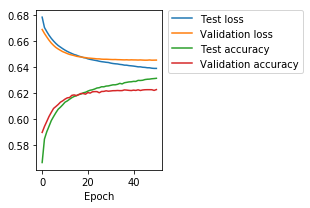
\includegraphics[width=157pt]{training}
\end{adjustbox}
\centering
\end{figure}

Each of the six trained models had very similar levels of accuracy and loss.  The mean validation accuracy was 62.10\% with 1 standard deviation of 0.08\%.  The mean validation loss was  0.64625 with 1 standard deviation of 0.00089.  This is a 0.4\% higher accuracy than any of the results achieved during the model selection, and I was pleasantly surprised.  The reason is because the training set is larger.

I selected the weights with the lowest loss from the 6 trials, and considered those the winner.

\section {Results}

Following the selection of model weights, I take the remaining 100,000 games which was excluded from the training rounds and use it to further validate and explore the results.  

\subsection {Benchmark model}

The naive bayesian classifier was trained using  using the same dataset available to neural network.  The overall accuracy was 56.7\%.

\subsection {Unoptimized Neural Network Accuracy}

\begin{figure}
\caption{Unoptimized Training Stats}
\label{figure:500training}
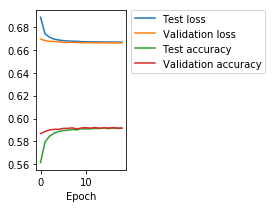
\includegraphics[width=136pt]{500training}
\end{figure}

The initial 2 layer, 500 perceptron network achieved 59.2\% accuracy on validation data, as show in Figure \ref{figure:500training}.  Through the choice of better hyperparameters, accuracy is increased by about 3\%.

\subsection {Optimized Neural Network Accuracy}

\begin{table}[h]
\caption{Model Accuracy}
\label{table:acc}
\centering
\begin{tabular}{lr}
\toprule
Game Mode & Percent \\
\midrule
Quick Match & 63.04\% \\
Hero League & 59.99\% \\
Team League & 59.87\% \\
Unranked Draft & 61.81\% \\
\midrule
Overall & 62.12\% \\
\bottomrule
\end{tabular}
\end{table}

On the holdout data, the trained model achieves 62.1\% accuracy.  Figure \ref{figure:training} includes the validation accuracy during training.  The validation set is different from the holdout data, but we expect that the accuracy should be about the same, which it is.  One thing we can do now is see which game modes are easier to predict.  As shown in Table \ref{table:acc}, \textit{quick match} games are easiest to predict, while \textit{team league} are the hardest.  This somewhat meets our expectations, as people will try harder to give themselves an advantage in ranked modes and not play heroes that put them at a large disadvantage.  However, \textit{quick match} is also the most frequently played mode and the match maker knows which heroes are going to be played, so it may be plausible for \textbf{Blizzard} to improve their matchmaker and make it harder for us to predict the winner.

\subsection{Calibration}

\begin{figure}[h]
\caption{Model Calibration}
\label{figure:calib}
\centering
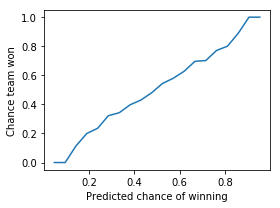
\includegraphics[width=\linewidth]{calibration}
\end{figure}

While predicting the eventual winner is ideal, it is simply not possible to know which team will win with complete certainty because either team can potentially win.  This means it is better for our model to tell us what the chances are that a particular team will win than to only guess which team will win.  After analyzing the results of the classifier, I found that it was not necessary to modify the output in any way.  I realized afterwards this is because of the loss function we are using, binary cross entropy, naturally causes the classifier to produce calibrated results.  We can see the model is well calibrated in Figure \ref{figure:calib}.  This means the output of the model directly tells us what are the chances that the first team will win.

\subsection{Confidence}

\begin{table}[h]
\caption{Model Confidence}
\label{table:confidence}
\centering
\begin{tabular}{lr}
\toprule
Minimum Confidence & Percent of Games \\
\midrule
100\% & 0.00\% \\
95\% & 0.04\% \\
90\% & 0.35\% \\
85\% & 1.42\% \\
80\% & 4.11\% \\
75\% & 9.54\% \\
70\% & 18.78\% \\
65\% & 32.63\% \\
60\% & 51.82\% \\
55\% & 74.72\% \\
50\% & 100.00\% \\
\bottomrule
\end{tabular}
\end{table}

One more thing we can consider is what percentage of games can be predicted with a given level of confidence.  For instance, we might ask what percent of games are played where one team is expected to win 75\% of the time or more.  As shown in Table \ref{table:confidence}, 9.54\% of games were predicted to have one team win 75\% of the time.  On the other hand, over 25\% of games are considered to be pretty even, with under 55\% confidence in choosing the correct winner.


\section{Conclusions}

\subsection{Reflection}
A model was successfully developed which accurately predicts more than 62\% of games, and can give reliable estimates on how likely a particular team is to win a given match.  The final model outperforms a bayesian fit by over 5\%.  This type of model could be useful in a number of ways, such as to improve matchmaking, or to develop a program to help choose the best heroes during the draft. 

Figures \ref{figure:match1} and \ref{figure:match2} contain sample matches from the validation set and their predicted results.

\begin{figure*}
\caption{Sample matches}
\label{figure:match1}
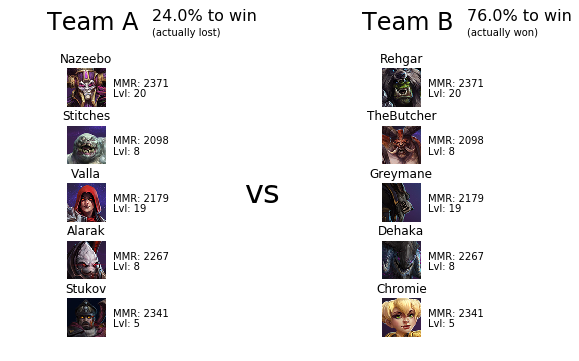
\includegraphics[width=\linewidth]{match1}
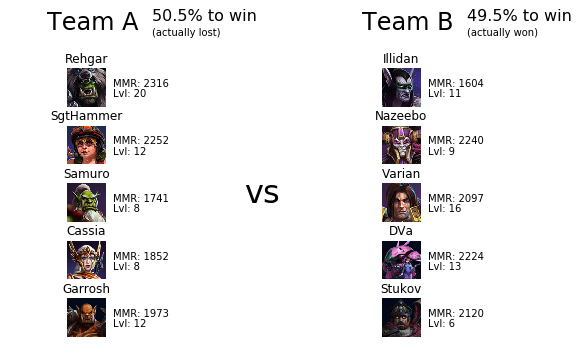
\includegraphics[width=\linewidth]{match2}
\centering
\end{figure*}

\begin{figure*}
\caption{More sample matches}
\label{figure:match2}
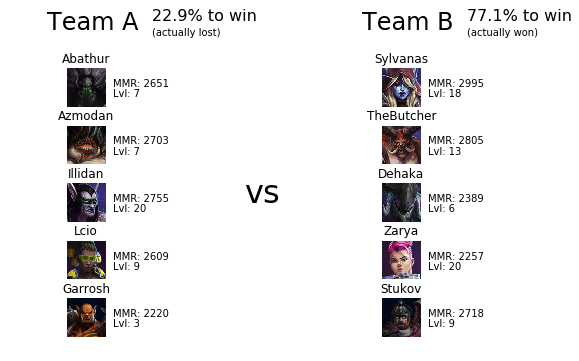
\includegraphics[width=\linewidth]{match3}
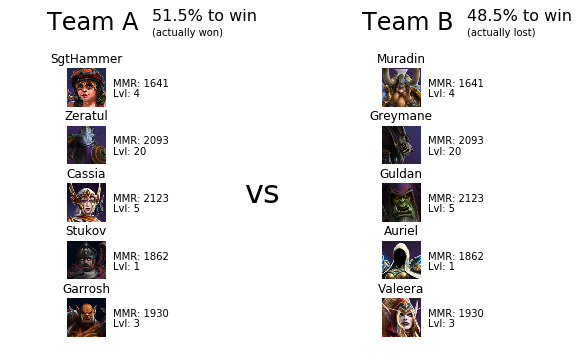
\includegraphics[width=\linewidth]{match4}
\centering
\end{figure*}


\subsection{Improvements}
Improvements could be made in a number of ways.  While PCA was not ultimately useful to me in my final model, I learned of something conceptually similar in Keras, called the Embedding layer, which could be used to change the hero ids, map id, and game modes into a dense vectors.  This was a big enough change that I did not pursue it for this project.  Another way to improve the results would be to try and use more data.  Over 10\% of the dataset was filtered out for various reasons, but the missing data could be filled in by using the mean of other players in the game.  We could also try to collect more than 30 days worth of games, however at some point we would then want to label each game with the \textit{Heroes of the Storm} patch version it was played on.






%\section{Discussion}

%A statement requiring citation \cite{Figueredo:2009dg}.


%----------------------------------------------------------------------------------------
%	REFERENCE LIST
%----------------------------------------------------------------------------------------

%\begin{thebibliography}{99} % Bibliography - this is intentionally simple in this template

%\bibitem[Figueredo and Wolf, 2009]{Figueredo:2009dg}
%Figueredo, A.~J. and Wolf, P. S.~A. (2009).
%\newblock Assortative pairing and life history strategy - a cross-cultural
 % study.
%\newblock {\em Human Nature}, 20:317--330.
 
%\end{thebibliography}

%----------------------------------------------------------------------------------------

\end{document}
